\documentclass[11pt]{article}

\usepackage[utf8]{inputenc}
\usepackage[T1]{fontenc}
\usepackage[margin=1in]{geometry}
\usepackage{graphicx}
\usepackage{booktabs,longtable,tabularx,array,multirow}
\usepackage{ragged2e}
\usepackage{pdflscape}
\usepackage{float}
\usepackage{placeins}
\usepackage{caption}
\usepackage{rotating}
\usepackage{makecell}
\usepackage[table]{xcolor}
\usepackage{xcolor}
\usepackage{amssymb}
\usepackage{microtype}
\usepackage{csquotes}
\usepackage{xurl}
\usepackage[hidelinks]{hyperref}


\usepackage{fontspec}
\usepackage{xeCJK}

\setmainfont{TeX Gyre Termes}
\setCJKmainfont{Noto Serif CJK SC}

% 日文单独指定字体
\newCJKfontfamily\japanesefont{Noto Serif CJK JP}


\usepackage[
    backend=biber,
    style=numeric-comp,
    sorting=none,
    sortcites=true,
    natbib=true,
    urldate=iso
]{biblatex}

\addbibresource{references.bib}
\title{Toward Objective Stroke Assessment: An Item-Level Analysis of Clinical Rating Scales for AI-Based Motion Analysis}

\author{
    Siqi Yang$^{1}$ \and
    Wenbo Qi$^{1}$ \and
    xxx$^{3}$ \and
    xxx$^{3}$ \and
    Baosheng Yu$^{1,2,3}$
}
\date{
    $^{1}$Lee Kong Chian School of Medicine, Nanyang Technological University, Singapore \\
    $^{2}$Centre of AI in Medicine, Nanyang Technological University, Singapore\\
    $^{3}$Rehabilitation Research Institute of Singapore, Nanyang Technological University, Singapore \\[1ex]
    \texttt{\{xxx,xxx\}@ntu.edu.sg, xxx@xxx.org}
}

\begin{document}
\maketitle

\begin{abstract}
Stroke is a leading cause of long-term disability worldwide, making objective assessment essential for consistent evaluation of motor function, personalized rehabilitation, and longitudinal recovery monitoring. Conventional clinical rating scales remain subjective and rely heavily on expert clinicians, limiting their consistency, scalability, and accessibility, particularly for frequent and remote assessments. 
Recent advances in computer vision, wearable sensing, and machine learning have enabled AI-based motion analysis for automated stroke assessment. However, most existing approaches formulate stroke assessment as end-to-end prediction of clinical scores, thereby inheriting the subjectivity of the underlying rating scales while providing limited insight into the quantitative movement features that underpin clinical assessment.
This survey presents a component-level framework that links clinical assessment with AI-based motion analysis. Rather than treating clinical scores as prediction targets, it examines how established rating scales can be decomposed into quantitative movement features that AI can objectively quantify. The survey reviews clinical rating scales, maps their assessment criteria to measurable movement features, and discusses sensing modalities and AI techniques for objective movement analysis. By explicitly linking clinical assessment with quantitative movement analysis, it provides a more interpretable and clinically grounded framework for AI-based stroke assessment and a foundation for developing next-generation objective clinical rating scales.
\end{abstract}


\section{Introduction}

Stroke is a leading cause of long-term disability worldwide, making accurate and objective assessment essential for personalized rehabilitation and longitudinal recovery monitoring. Across the stroke continuum, human movement serves as a key functional biomarker, reflecting both pre-stroke risk and post-stroke impairment and recovery. Consequently, objective quantification of human movement provides a natural foundation for stroke assessment. However, current clinical practice relies predominantly on standardized rating scales based on clinician observation and qualitative judgment rather than quantitative analysis of movement. Widely used scales, such as the Fugl-Meyer Assessment (FMA), summarize motor performance through coarse ordinal ratings that are inherently subjective, susceptible to inter-rater variability, and dependent on trained clinicians, limiting their scalability and suitability for frequent or continuous assessment.

Recent advances in computer vision, wearable sensing, and machine learning have enabled AI-based motion analysis to quantify human movement from video and wearable sensor data. Most existing approaches formulate stroke assessment as end-to-end prediction of clinical scores, learning direct mappings from raw motion signals to clinician-assigned ratings without explicitly modeling the quantitative movement features that underpin clinical assessment. Consequently, these models inherit the subjectivity and limited granularity of the target rating scales while providing little insight into how specific movement abnormalities contribute to clinical outcomes. More fundamentally, treating clinical scores as the primary prediction target overlooks the fact that these scores are higher-level clinical interpretations of underlying movement characteristics. As illustrated in Figure~\ref{fig:figure1}, effective AI-based stroke assessment should therefore explicitly quantify clinically meaningful movement features and relate them to clinical evaluation, rather than directly predicting clinical scores alone. This perspective enables more interpretable representations of motor dysfunction and better supports rehabilitation planning, longitudinal monitoring, and clinical decision-making.

\begin{figure}[!t]
    \centering
    \includegraphics[width=0.9\linewidth,height=0.55\linewidth]{figure1.pdf}
    \caption{\textbf{Overview of the component-level framework linking clinical rating scales with AI-based motion analysis.} Clinical rating scales grade observed task performance against ordinal scoring criteria (left). Instead of directly predicting clinical scores, the framework maps the observable part of each criterion to five families of quantitative movement features (centre; Section~\ref{sec:framework}) and combines task-specific measures into a movement profile that supports criterion scoring, longitudinal monitoring and clinical decisions (right). Some features quantify a criterion directly, such as Timed Up and Go (TUG) duration; others only indicate a construct, such as trunk displacement during reaching as a possible sign of compensation. The amount of assistance, verbal cues, applied force, tone and self-report are not captured by motion features and require other sources. Clinical use requires analytical, task-level and clinical-construct validity and clinical utility. The movement profile and monitoring trend are illustrative.}
    \label{fig:figure1}
\end{figure}


Motivated by this perspective, this survey introduces a component-level framework that bridges established clinical assessment with AI-based motion analysis. Rather than treating clinical scores as end-to-end prediction targets, it investigates how widely used stroke assessment scales can be decomposed into quantitative movement features that AI can objectively quantify. Specifically, the survey reviews established clinical rating scales, maps their assessment criteria to quantitative movement features, and systematically examines AI-based motion analysis methods through this lens. It further evaluates the extent to which current approaches capture clinically meaningful aspects of motor function and identifies important gaps between clinical assessment requirements and existing computational capabilities. By explicitly connecting clinical evaluation to quantitative movement analysis, this survey provides a roadmap for developing more interpretable, clinically grounded, and objective AI systems for stroke assessment.

The remainder of this paper is organized as follows. Section~\ref{sec:background} provides the background on stroke assessment and AI-based motion analysis. Section~\ref{sec:scales} reviews commonly used clinical rating scales and analyzes their constituent assessment components from a motion analysis perspective. Section~\ref{sec:framework} presents the proposed component-level framework for objective AI-driven stroke assessment. Finally, Section~\ref{sec:challenge} discusses the key challenges, emerging opportunities, and future research directions toward objective and interpretable AI-driven stroke assessment.


\section{Background and Preliminaries}
\label{sec:background}

Stroke results from cerebral ischaemia or haemorrhage. Motor impairment can disrupt voluntary control, coordination, balance, gait and upper-limb function, limiting mobility and daily activities \cite{WHO2025StrokeFactSheet,S1VADoD2024StrokeRehab}. The purpose of assessment changes along the care pathway. In acute care, the National Institutes of Health Stroke Scale (NIHSS) grades neurological severity and tracks early change \cite{S1Prabhakaran2026AHAASAAIS,ScaleBrott1989NIHSS}. During rehabilitation and after discharge, clinicians assess motor impairment, balance, gait, upper-limb activity and independence to guide goal setting and follow-up \cite{S1Winstein2016AHAASARehab,S1VADoD2024StrokeRehab,S1NICE2023NG236}. Ordinal ratings, times, speeds, distances and counts describe complementary aspects of recovery. Each requires its own interpretation \cite{ScaleHarrison2013Clinimetric,CoreKwakkel2017SRRRSensorimotor,CoreVanCriekinge2024SRRRBalanceMobility}.

We distinguish four levels of description. The \emph{clinical construct} is what the scale measures, such as standing balance. A \emph{score-defining criterion} distinguishes adjacent grades, for example by whether a patient uses their hands to stand up. The \emph{observable movement information} in a criterion may include hand use, duration or loss of balance. A criterion can also depend on information outside the recording. \emph{Computational features} are quantities derived from motion signals, such as gait speed, joint angle or trunk displacement. A feature may quantify a criterion directly, indicate it indirectly or have no counterpart in any scale.

Pose estimation recovers body landmarks and trajectories from RGB or depth video. These trajectories yield estimates of timing, displacement and joint angles for visible segments. Accuracy depends on viewpoint, calibration, occlusion and tracking \cite{S3Luvizutto202234115576,S3Lonini202235224426,S3John202437682075}. Inertial measurement units (IMUs) record segment acceleration and angular velocity even outside the camera's field of view \cite{S3OBrien202236304845,Yang2013SpatiotemporalGait}. Neither modality records force, muscle tone or what the patient perceives. The motion signals yield five feature families that describe how a movement is executed (Section~\ref{sec:framework}).

\section{Clinical Rating Scales: A Motion Analysis Perspective}
\label{sec:scales}

\subsection{Review Methodology}

\paragraph{Tool library.} We built a purposive library of standardised motor and mobility assessments to map their scoring criteria (Fig.~\ref{fig:figure2}). The guideline search covered adult-stroke guidelines, standards and consensus documents. Eligible documents made assessment recommendations and had a complete English text. We searched PubMed, Embase, the Guidelines International Network, TRIP, World Health Organization resources, issuing-body websites and reference lists. The search ended in May 2026, with no subsequent update. For documents already published online by that date, we cite the final print version. One example is the 2026 AHA/ASA acute ischaemic stroke guideline, first published online in January 2026. For coding and verification, we continued to consult web-based scoring manuals and tool specifications until August 2026, as indicated by their access dates.

Two reviewers screened records independently and resolved disagreements by consensus. They excluded 13 of the 41 full-text documents, seven because a complete English text was unavailable. The 28 included guidelines covered nine regions and named 37 tools (Supplementary Table~\ref{tab:s1_guidelines_compact}). We searched for each tool's full name and read the passage to confirm the match. A full-name mention qualified a tool for inclusion even without a formal recommendation. We did not grade recommendation strength.

A supplementary search identified standardised tools used in stroke research but absent from the included guidelines. PubMed-indexed stroke studies published in 2022--2026 and citation tracking yielded 240 candidates. Of these, 184 had support from at least one meta-analysis, systematic review or multicentre study. We checked the source specifications and scoring manuals in 58 reports and retained 22 tools. Retention depended on their relevance to motor and mobility assessment and whether we could verify their scoring specifications. We did not record individual reasons for excluding the other 162 leads, making this the least reproducible step. Only an excluded non-English guideline recommended the Modified Tardieu Scale. As an exception to the guideline language rule, we included the scale using its English specification \cite{S2RehabMeasuresModifiedTardieu}.

We merged walking speed into the 10-Metre Walk Test (10MWT). We also removed two records that lacked standardised motor scoring (observational gait analysis and the Frenchay Activities Index). The final library comprised 57 tools. Supplementary Data~1 provides the search strings and screening logs.

\paragraph{COA classification.} We applied clinical outcome assessment (COA) definitions according to how each tool generates a score \cite{FDANIH2016BESTCOA,Walton2015COAConceptualFoundation}. Performance outcomes (PerfO) use measured quantities or observable task outcomes. Clinician-reported outcomes (ClinRO) require judgement of assistance, supervision, safety, movement normality, examination signs, recovery stage or global status, even on a standardised task.

Under this operational classification, the library comprised 16 PerfO tools, 33 ClinRO tools, six patient-reported outcome (PRO) tools and two tools with mixed outputs. The Wolf Motor Function Test (WMFT) combines timed and strength outputs (PerfO) with its Functional Ability Scale (ClinRO). The Rivermead Mobility Index (RMI) combines 14 self-reported items with one observed item (Supplementary Table~\ref{tab:supplementary_tool_library_clinical}).

A task-based interpretation, common in regulatory use, treats an instructed standardised task as PerfO when the score derives from the performance, regardless of who rates it. This would move 17 ClinRO tools into PerfO, among them the BBS, Mini-BESTest, DGI, ARAT and FMA. The mixed-output WMFT would also qualify. It yields 34 PerfO, 16 ClinRO, six PRO and one mixed tool (Supplementary Table~\ref{tab:supplementary_tool_library_clinical}). Tools graded by examiner-applied force or touch, tone or reflex examination, recovery stage, global status or usual performance remain ClinRO under both readings.

We retained the operational classification to identify grades that require rater judgement. Neither classification affected availability or computability coding.

\paragraph{Mapping entries.} We mapped each tool at the level at which its scoring rules differed, yielding 196 entries. Thirteen tools had item-specific ordinal criteria and contributed 129 item-level entries. Examples include the Berg Balance Scale (BBS), Trunk Impairment Scale (TIS), Mini-Balance Evaluation Systems Test (Mini-BESTest) and Tinetti Performance-Oriented Mobility Assessment (POMA). Ten tools shared criteria within subtests and contributed 33 subtest-level entries. Examples include the Action Research Arm Test (ARAT), Fugl-Meyer Assessment (FMA) and WMFT.

We mapped 34 tools as a whole (34 entries). Most yielded a single time, distance, count or category, as in the 10MWT, Timed Up and Go (TUG) and Functional Ambulation Category (FAC). This group also included global ratings and questionnaires. We mapped some item-structured instruments as whole tools, including the Function in Sitting Test, Community Balance and Mobility Scale and Chedoke Arm and Hand Activity Inventory. We therefore report tool-weighted proportions alongside entry counts. For multi-domain tools, we mapped only motor and mobility content, using the versions listed in Supplementary Table~\ref{tab:supplementary_tool_library_clinical}.

\paragraph{Coded attributes.} We coded five attributes for each entry using the official scoring criteria. We included tool-wide rules whenever they changed an item's score. Supplementary Data~1 provides the rules and worked examples.

(i) We marked a \emph{movement component} only when the criteria graded performance in that component. A task could require a component without grading it.

(ii) We recorded each \emph{information type} used to distinguish grades. The types covered kinematics or movement quality, time, distance or count, assistance or supervision, and safety judgement. They also included verbal cues or responses, applied force or touch, tone or reflexes, and self-report. An entry could have more than one type.

(iii) We assessed \emph{availability from ordinary video} assuming one RGB camera framed the task as administered. We coded an entry as Full if all grade-defining information was visible in an adequate recording. This included visible assistance or support. An examiner's presence, guarding, standard instructions or visible physical help did not by itself lower the code. We coded an entry as Partial if only some grade-defining information was visible. Missing information could include how much help the examiner gave, force or resistance applied during examination, events confirmed by touch, verbal cues or responses, or judgements with no visible trace. It could also include usual performance outside the recording. We coded an entry as None if its score did not derive from visible performance. Examples include patient report, reflexes, and tone or force assessed by touch or instrument.

For example, BBS standing items graded partly by supervision were Full because the instability that prompts supervision is visible. BBS sit-to-stand was Partial because lower grades distinguish minimal assistance from moderate or maximal assistance. Clinician ratings of observed or usual performance were Partial in the Barthel Index (BI), Functional Independence Measure (FIM) and modified Rankin Scale. RMI questionnaire items were None because patients supply the answers. This code applies to video alone. An interview can supply patient-reported information for use alongside video-derived measures. We repeated the availability coding under two alternative recording conditions. One added audio to RGB video. The other assumed a routine recording with one viewpoint per task, no hand close-up, no added calibration reference and no simultaneous second view.

(iv) We linked each entry to the \emph{computational feature families} that could quantify the observable part of its criteria (Section~\ref{sec:framework}).

(v) We coded the \emph{computability} of the visible criteria according to the least computable grade boundary. We used Direct if every grade boundary specified a threshold for time, distance, count, angle or displacement, or a discrete visible event. Events included task completion, a step, contact, use of the hands, an aid or physical help, and a fall. We used Proxy when at least one boundary graded the degree of a named observable property, such as steadiness, path deviation, symmetry or a listed compensation. A feature can target that property, but its grade thresholds require validation against rater scores. We used Judgement when at least one boundary required an overall clinical judgement without naming a single property. Examples include a normal or abnormal movement pattern, recovery stage and global disability. For Partial entries, computability applied only to the visible part.

Availability describes what a rater could observe. Computability describes whether a computed quantity could reproduce a grade boundary. Neither code establishes measurement accuracy or validates automated scoring. A feature-family link identifies a class of measures and does not establish the validity of an individual feature. For each entry, Supplementary Data~1 gives the task, full scoring criteria, coding rationale and recording requirements. It also identifies information that video cannot supply and gives an alternative source.

\paragraph{Verification.} We checked availability codes in three stages. Supplementary Data~1 traces each entry through all three.

First, two reviewers independently coded the initial 193 entries. The first reviewer classified 82 as Full, 82 as Partial and 29 as None. Agreement was 77.2\% (Cohen's $\kappa$ = 0.63). With Full, Partial and None treated as ordered categories, linearly weighted $\kappa$ was 0.68. Of the 44 disagreements, 40 concerned the distinction between Partial and Full. The reviewers checked the scoring manuals and changed 34 codes by consensus, yielding 115 Full, 53 Partial and 25 None.

Second, one coder documented the rules and applied them across tools. A check of tool versions, outputs and scoring manuals led to the exclusion, splitting or redefinition of 12 previously checked entries. This step also added or redefined 15 entries. The resulting set comprised 196 entries (106 Full, 62 Partial and 28 None). Of these, 181 had been checked in the initial exercise, and 54 of those had changed code since consensus. The other 15 had not been checked independently.

Third, we revised the availability rule so that visible assistance alone no longer lowered the code. The same coder re-examined all 196 entries against the scoring manuals, changed 36 availability codes and 19 information types, and flagged 22 borderline decisions. The final counts were 134 Full, 36 Partial and 26 None. Of the 181 previously checked entries, 129 retained their consensus code. The same coder assigned movement components, information types, feature-family links and computability. The agreement statistics apply only to the two reviewers' initial availability ratings under the earlier rule (Section~\ref{sec:limitations}).

\begin{figure}[!htbp]
    \centering
    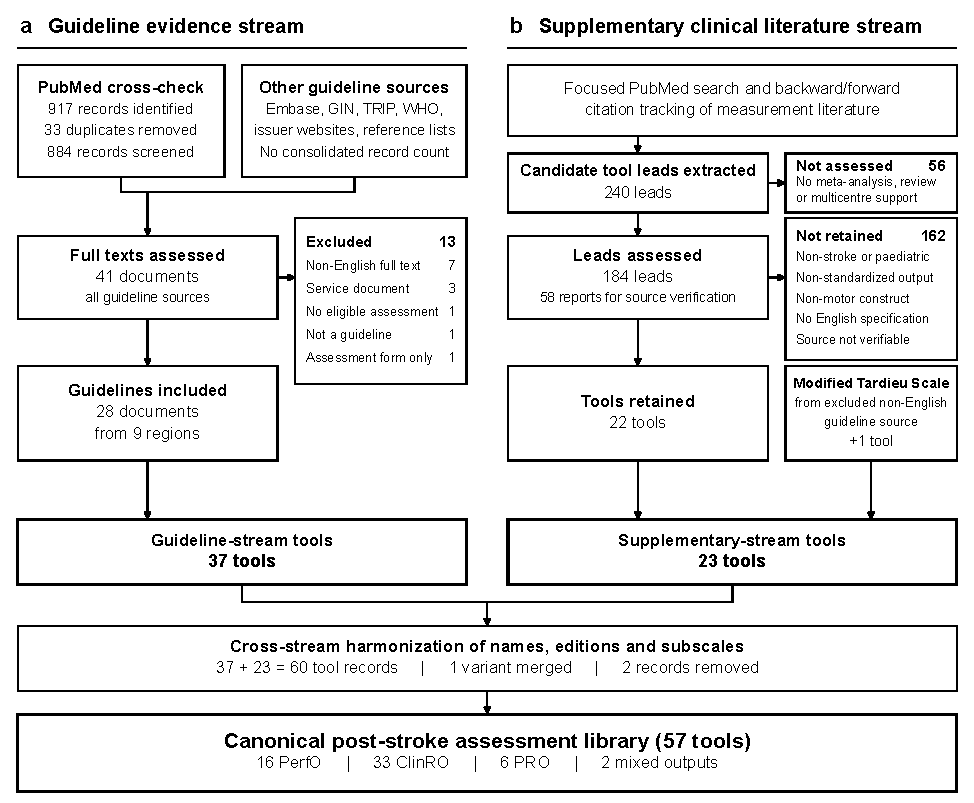
\includegraphics[
        height=0.58\textheight,
        width=\linewidth,
        keepaspectratio
    ]{figure2.pdf}
    \captionsetup{justification=raggedright,singlelinecheck=false}
    \caption{\textbf{Construction of the assessment-tool library.} This library-level diagram does not trace individual records through the PRISMA stages. \textbf{a,} Guideline record counts cover the PubMed cross-check only. Full-text assessment pooled all sources. \textbf{b,} The supplementary stream lacked exclusion counts by reason. Harmonisation merged walking speed into the 10MWT and removed two records without standardised motor scoring. PerfO, ClinRO and PRO denote performance, clinician-reported and patient-reported outcomes (Section~\ref{sec:scales}). GIN denotes the Guidelines International Network, TRIP the TRIP Database and WHO the World Health Organization.}
    \label{fig:figure2}
\end{figure}


\subsection{Clinical Rating Scales}
\label{sec:clinical_rating_scales}

Table~\ref{tab:representative_scales_compact} summarises 13 representative tools. Of these, 11 reflect priorities from the three Stroke Recovery and Rehabilitation Roundtable (SRRR) consensus rounds \cite{CoreKwakkel2017SRRRSensorimotor,CoreKwakkel2019SRRRUpperLimb,CoreVanCriekinge2024SRRRBalanceMobility}. Guidelines supplied the TUG for transitional mobility and the BI for daily activities \cite{S1Winstein2016AHAASARehab,S1VADoD2024StrokeRehab}. Outputs include ordinal grades, measures of time, speed or distance, and categories of independence.

We grouped recurrent item content into six movement components. Three concern joint mobility and range of motion, muscle strength and force production, and coordination and selective motor control. The other three cover balance and postural control, manual dexterity and upper-limb task execution, and gait and functional mobility. Movement quality and compensation can modify performance in any component. A patient may achieve the same task outcome through restitution or compensation \cite{Levin2009RecoveryCompensation,CoreKwakkel2019SRRRUpperLimb}. The grouping draws on the International Classification of Functioning, Disability and Health (ICF) and SRRR domains \cite{WHO2001ICF,Cieza2019ICFLinking,CoreKwakkel2017SRRRSensorimotor}. It supports cross-scale comparison but has yet to be validated as a taxonomy.

Table~\ref{tab:representative_scales_compact} marks a component only when the scoring criteria grade it. Walking 10~m requires balance, for example, but the 10MWT records speed. Gait is therefore its only score-defining component. Postural control determines most BBS and Mini-BESTest grades, whereas the ARAT does not grade it.

Scales that share a movement component can still grade different aspects of performance. The FMA upper-extremity motor subscale (FMA-UE) grades synergy-dependent and selective movement \cite{ScaleFuglMeyer1975PhysicalPerformance,ScaleSee2013StandardizedFMA}. The ARAT grades completion of 19 tasks \cite{ScaleYozbatiran2008StandardizedARAT}. A patient who completes a task through trunk or shoulder compensation can therefore score on an activity measure without regaining motor control \cite{Levin2009RecoveryCompensation,Santisteban2016UpperLimbOutcome}. The TIS, BBS and Mini-BESTest all grade postural control but differ in the body segment, task context and information used for scoring \cite{ScaleVerheyden2004TIS,ScaleBerg1992BalanceValidation,ScaleFranchignoni2010MiniBESTest}.

Lower-limb tools grade impairment (FMA lower-extremity subscale, FMA-LE), walking independence (FAC), speed (10MWT) or endurance (6-Minute Walk Test, 6MWT). The Dynamic Gait Index (DGI) and TUG address adaptive and transitional mobility, respectively \cite{ScaleHolden1984FAC,ScaleCheng2020StrokeWalkTests,ScaleAn2017DGIStroke,ScaleNg2005TUGStroke}. SRRR considers the 10MWT, 6MWT and DGI untestable when the FAC is below 3 \cite{CoreVanCriekinge2024SRRRBalanceMobility}. What can be observed therefore depends on the patient's walking independence. In the NIHSS and BI, only the motor and mobility items relate to movement \cite{ScaleBrott1989NIHSS,ScaleMahoney1965Barthel}.

% Main-text Table 1: movement components required by representative scales.
% Required packages: booktabs, array, ragged2e, graphicx (for \rotatebox).

\begin{table}[!htbp]
\centering
\caption{Score-defining movement components of representative post-stroke scales. A component is marked only when the scoring criteria grade it; shared components do not make scores interchangeable.}
\label{tab:representative_scales_compact}
\begingroup
\newcommand{\mcmark}{\(\bullet\)}
\setlength{\tabcolsep}{4pt}
\renewcommand{\arraystretch}{1.1}
\small
\begin{tabular}{@{}l l l *{7}{c}@{}}
\toprule
 & & & \multicolumn{6}{c}{\textbf{Movement component}} & \textbf{Modifier} \\
\cmidrule(lr){4-9}\cmidrule(l){10-10}
\textbf{Scale} & \textbf{COA} & \textbf{Score output} & ROM & S/F & Coord. & Bal. & Dex. & Gait & Q/C \\
\midrule
\multicolumn{10}{@{}l}{\textit{Upper limb}} \\
FMA-UE & ClinRO & Ordinal (0--66) & \mcmark & \mcmark & \mcmark &  & \mcmark &  & \mcmark \\
ARAT & ClinRO & Ordinal (0--57) &  &  & \mcmark &  & \mcmark &  & \mcmark \\
\midrule
\multicolumn{10}{@{}l}{\textit{Trunk and balance}} \\
TIS & ClinRO & Ordinal (0--23) &  &  & \mcmark & \mcmark &  &  & \mcmark \\
BBS & ClinRO & Ordinal (0--56) &  &  &  & \mcmark &  & \mcmark & \mcmark \\
Mini-BESTest & ClinRO & Ordinal (0--28) & \mcmark &  &  & \mcmark &  & \mcmark & \mcmark \\
\midrule
\multicolumn{10}{@{}l}{\textit{Lower limb and mobility}} \\
FMA-LE & ClinRO & Ordinal (0--34) & \mcmark & \mcmark & \mcmark &  &  &  & \mcmark \\
DGI & ClinRO & Ordinal (0--24) &  &  & \mcmark & \mcmark &  & \mcmark & \mcmark \\
FAC & ClinRO & Category (0--5) &  &  &  & \mcmark &  & \mcmark &  \\
10MWT & PerfO & Speed (m/s) &  &  &  &  &  & \mcmark &  \\
6MWT & PerfO & Distance (m) &  &  &  &  &  & \mcmark &  \\
TUG\textsuperscript{a} & PerfO & Time (s) &  &  &  &  &  & \mcmark &  \\
\midrule
\multicolumn{10}{@{}l}{\textit{Global outcome (movement-related items only)}} \\
NIHSS & ClinRO & Ordinal (0--42) &  & \mcmark & \mcmark &  &  &  &  \\
BI\textsuperscript{a} & ClinRO & Ordinal (0--100) &  &  &  &  &  & \mcmark &  \\
\bottomrule
\end{tabular}

\vspace{3pt}
\begin{minipage}{\linewidth}
\footnotesize
\textit{Notes.} \(\bullet\), at least one item's criteria grade performance in that component (rules in Supplementary Table~\ref{tab:supplementary_tool_library_motion}); components a task requires without changing the grade are not marked, such as balance in the time-scored 10MWT and TUG or trunk range in TIS items graded by completion, symmetry and compensation. Gait includes transfers and stepping (BBS, BI). S/F covers FMA items graded against examiner resistance and, for the NIHSS, holding a limb against gravity. Q/C, movement quality and compensation, is a cross-component modifier marked only when criteria grade quality, abnormal synergy or compensation. NIHSS: motor and limb-ataxia items; BI: mobility items. \textsuperscript{a}Guideline-supported tools added to the 11 SRRR-priority tools for transitional mobility (TUG) and daily activities (BI). COA is an operational classification under FDA--NIH definitions (Section~\ref{sec:scales}) \cite{FDANIH2016BESTCOA,Walton2015COAConceptualFoundation}; under a task-based reading, the task-rated ClinRO tools here (FMA-UE, ARAT, TIS, BBS, Mini-BESTest, FMA-LE, DGI) would be PerfO (Supplementary Table~\ref{tab:supplementary_tool_library_clinical}); components were informed by the ICF, guidelines and SRRR domains \cite{WHO2001ICF,S1Winstein2016AHAASARehab,S1VADoD2024StrokeRehab,S1NICE2023NG236,CoreKwakkel2017SRRRSensorimotor,CoreKwakkel2019SRRRUpperLimb,CoreVanCriekinge2024SRRRBalanceMobility}.
ROM, joint mobility and range of motion; S/F, strength and force production; Coord., coordination and selective motor control; Bal., balance and postural control; Dex., manual dexterity and upper-limb task execution; Gait, gait and functional mobility.
10MWT, 10-Metre Walk Test; 6MWT, 6-Minute Walk Test; ARAT, Action Research Arm Test; BBS, Berg Balance Scale; BI, Barthel Index; ClinRO, clinician-reported outcome; COA, clinical outcome assessment; DGI, Dynamic Gait Index; FAC, Functional Ambulation Category; FMA-LE/UE, Fugl--Meyer Assessment lower/upper extremity; Mini-BESTest, Mini-Balance Evaluation Systems Test; NIHSS, National Institutes of Health Stroke Scale; PerfO, performance outcome; TIS, Trunk Impairment Scale; TUG, Timed Up and Go.
\end{minipage}
\endgroup
\end{table}

\clearpage

\section{Toward Objective AI-Driven Stroke Assessment}
\label{sec:framework}
\subsection{From Clinical Scores to Computational Feature Families}

AI models can estimate selected clinical scores from motion data \cite{Lee2021SmartphoneVideoAmbulation,Formstone2021IMUMMG,Zamin2023BIONICS,Li2017IMUEMGMotorEvaluation}. A depth-camera study reported accuracies of 65--87\% across 13 FMA-UE items \cite{Kim2016KinectFMA}. Yet the same grade can reflect limited excursion, slowness, asymmetry, instability or compensation. SRRR recommends kinematic and kinetic measures alongside clinical scales \cite{CoreKwakkel2019SRRRUpperLimb,CoreVanCriekinge2024SRRRBalanceMobility}.

Our mapping follows the sequence clinical item $\rightarrow$ scoring criterion $\rightarrow$ observable information $\rightarrow$ computational feature $\rightarrow$ clinical interpretation. In BBS sit-to-stand, video can show hand push-off, transition time and instability. Lower grades also depend on how much help the examiner gives, which motion alone cannot quantify. In the TUG, onset and return to sitting define the score. Phase durations and turning steps add detail.

A movement component can yield several feature families, and a feature can apply to several components. A gait item, for example, yields temporal, spatial and relational measures. The same joint-angle computation can quantify FMA range of motion or describe trunk inclination during TIS items.

Features vary in their correspondence to scoring criteria (Table~\ref{tab:computational_feature_families}). Test time, walking speed, reach distance or active joint excursion may measure the criterion directly. Joint coupling or trunk displacement may indicate abnormal synergy or compensation, but interpreting the pattern still requires clinical judgement.

Measuring distance or joint angles requires calibration, an aligned view and reliable tracking. Video cannot capture force, passive tone, reflexes, sensation, pain or self-report. Parts of the examination may still be visible, such as the angle of a catch during passive stretch.

% Main-text Table 2: computational feature families (revised round 4).
% Required packages: booktabs, tabularx, array, ragged2e.

\begin{table*}[t]
\centering
\caption{Computational feature families: the scoring criteria they quantify directly and the constructs they only indicate.}
\label{tab:computational_feature_families}
\setlength{\tabcolsep}{4pt}
\renewcommand{\arraystretch}{1.15}
\small
\begin{tabularx}{\textwidth}{@{}
>{\RaggedRight\arraybackslash}p{0.13\textwidth}
>{\RaggedRight\arraybackslash}p{0.15\textwidth}
>{\RaggedRight\arraybackslash}X
>{\RaggedRight\arraybackslash}p{0.17\textwidth}
>{\RaggedRight\arraybackslash}p{0.17\textwidth}
>{\RaggedRight\arraybackslash}p{0.10\textwidth}
@{}}
\toprule
\textbf{Feature family} & \textbf{Example variables} & \textbf{Quantifies a scoring criterion directly} & \textbf{Indicates only (validation needed)} & \textbf{Requirements for video} & \textbf{Other sensors} \\
\midrule
Temporal and event & Duration, count, cadence, phase timing & Test time (10MWT, TUG); repetitions; time-limited holds (TIS static items) & Overall mobility or fall risk inferred from test time & Visible task onset and end; adequate frame rate & IMU, pressure \\
Spatial and trajectory & Path length, displacement, endpoint error, foot clearance & Distance walked (6MWT); reach distance (FRT); trunk-displacement thresholds (TIS) & Dysmetria or motor-planning deficits inferred from path shape & Scale calibration from a known distance; whole path in view & IMU, depth camera, robot \\
Joint and segment kinematics & Joint angle, active ROM, angular velocity & Active range where criteria grade range (FMA; Mini-BESTest rise to toes) & Abnormal synergy; selective motor control & View aligned with the plane of motion; 3D estimation for out-of-plane motion & IMU, depth camera, exoskeleton \\
Inter-segment and relational & Bilateral symmetry, phase difference, joint coupling, trunk--limb relation & Use of arm or rail support where criteria define it (TIS, POMA) & Coordination; compensation; interlimb control & Both sides and relevant segments visible; synchronised tracking & Multi-IMU, depth camera \\
Trajectory-derived quality & Smoothness, jerk, movement units, path efficiency & Rarely graded by scoring criteria (6 entries in 6 tools; Fig.~\ref{fig:video_availability}c) & Movement quality; restitution versus compensation & Low tracking noise; adequate frame rate; reported filtering & IMU, robot, motion capture \\
\midrule
\textit{Non-kinematic information} & \textit{Force, passive tone, reflex, sensation, pain, self-report; amount of assistance, verbal cues and safety judgements} & \textit{Not quantified by motion features} & -- & \textit{Force, tone, reflexes, sensation and self-report not available from video; assistance visible as events but its amount only partly; verbal cues need audio} & \textit{Force or pressure, EMG/MMG, audio, clinical examination, interview} \\
\bottomrule
\end{tabularx}

\vspace{3pt}
\begin{minipage}{\textwidth}
\footnotesize
\textit{Notes.} \textit{Quantifies a scoring criterion directly}: the measure is the graded quantity, so measurement accuracy is the main requirement. \textit{Indicates only}: the measure informs but does not establish a construct graded by clinical judgement or lying outside the scale, and needs construct validation. One variable can fall in both columns (an active joint angle quantifies graded range but only indicates abnormal synergy), and one item can yield measures from several families. The last row marks an observability boundary, not a sixth family. Entry-level computability (Direct, Proxy or Judgement) is given in Supplementary Table~\ref{tab:supplementary_tool_library_motion}. Abbreviations follow Table~\ref{tab:representative_scales_compact}; EMG, electromyography; FRT, Functional Reach Test; IMU, inertial measurement unit; MMG, mechanomyography; POMA, Performance-Oriented Mobility Assessment; ROM, range of motion.
\end{minipage}
\end{table*}


Of 196 entries, video could provide all score-defining information for 134 (68\%), some for 36 (18\%) and none for 26 (13\%) (Fig.~\ref{fig:video_availability}a). The 104 entries graded solely on movement, time, distance or count were Full by definition.

In 19 tools, 55 entries combined movement with assistance, supervision, safety or verbal information. Of these, 30 were Full because the relevant assistance, support or instability was visible. The other 25 were Partial. Their grades depended on the amount of assistance (nine), verbal cues or responses (eight), usual performance outside the recording (six) or a supervision judgement with no visible trace (two). Of the 17 entries graded partly by examiner-applied force, tone or reflexes, 11 were Partial and six were None. None of the 20 entries that used patient report was Full.

Item-level balance scales such as the TIS, POMA, Mini-BESTest and BBS contribute many entries (Fig.~\ref{fig:video_availability}d). Giving each tool equal weight reduced the fully available share to 53\% and raised the unavailable share to 18\% (Fig.~\ref{fig:video_availability}b). The Rivermead Mobility Index contributed 15 entries (8\% of the total), including 14 of the 26 unavailable entries. After its exclusion, 133 of 181 entries (73\%) were Full, 36 (20\%) were Partial and 12 (7\%) were None.

Among 176 entries based on observed performance or examination, 134 (76\%) were Full, 36 (20\%) Partial and six (3\%) None. All six unavailable entries depended on force, tone or reflexes.

Adding audio changed five Partial entries to Full (139 Full, 71\%). These lacked only a verbal cue or response, as in BBS transfers and turns or the Mini-BESTest dual task. The other 17 entries needing audio also required an examiner's record, interview or daily-life information (Supplementary Data~1).

With one routine viewpoint per task, 30 entries from 17 tools changed from Full to Partial. This left 104 Full entries (53\%, or 34\% with equal tool weighting). Of the affected entries, 14 required a close-up of finger or grasp detail, as in the ARAT pinch subscale and Nine-Hole Peg Test. Seven used a ruler to measure distances in centimetres, as in the Functional Reach Test. Another seven combined frontal-plane deviation or weight distribution with sagittal timing or extension, as in the FGA walking items. The 2MWT and 6MWT required locating the end of a partial lap on a course extending beyond one field of view. Combining routine camera set-up with audio yielded 109 Full entries (56\%). A Full code therefore depends on how the task is recorded.

Of 134 fully available entries, 61 (46\%) were Direct. Another 57 (43\%) were Proxy because a boundary graded a visible property, such as steadiness or symmetry, without specifying a threshold. The remaining 16 (12\%) required overall Judgement, as when DGI or FGA walking items grade gait as normal or abnormal. The 104 entries that were Full by construction also spanned all three categories (49 Direct, 44 Proxy, 11 Judgement).

Across the library, 61 of 196 entries (31\%, or 34\% with equal tool weighting) were both fully available and directly computable. They came from 27 tools. In 16 tools, every entry met both conditions. Most were timed, counted or distance tests, including the 10MWT, TUG, Box and Block Test, Nine-Hole Peg Test and Manual Function Test. Among the 36 Partial entries, the visible part was Direct in 21, Proxy in nine and Judgement in six. Direct examples included hand or rail use and the occurrence of help in the Ability for Basic Movement Scale and BI.

Fully available Proxy and Judgement entries (73) outnumbered Partial and None entries combined (62). Grading a visible movement was therefore a more frequent obstacle than missing information. Learning or validating thresholds against rater grades also carries forward disagreements between raters (Supplementary Table~\ref{tab:supplementary_tool_library_motion}).

Temporal and event measures had anchors in 153 entries across 42 tools, and spatial and trajectory measures in 81 entries across 24 tools. Joint and segment kinematics had anchors in 52 entries across 21 tools, and inter-segment and relational measures in 46 across 19. Only six entries across six tools anchored trajectory-derived quality measures (Fig.~\ref{fig:video_availability}c). Few scale criteria therefore provide a reference for features such as smoothness or jerk (Section~\ref{sec:constructs}).

\begin{figure}[!htbp]
    \centering
    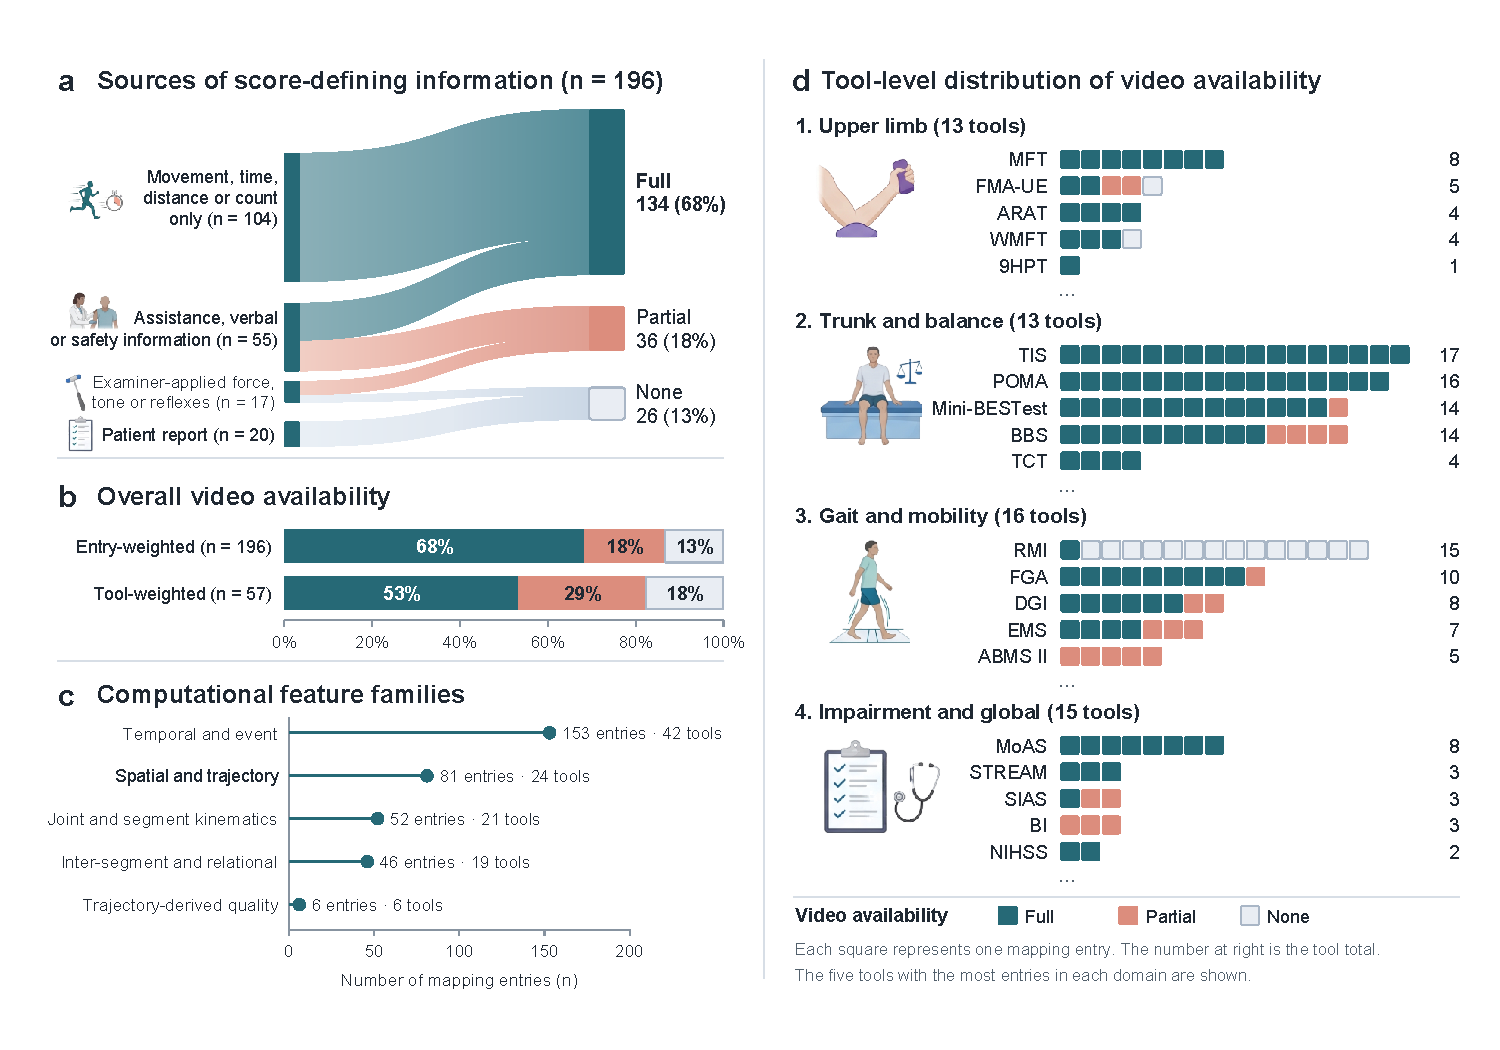
\includegraphics[width=\linewidth]{figure3.pdf}
    \caption{\textbf{What ordinary video can provide for scale scoring.} \textbf{a,} Scoring information (left) and its availability from video (right) for 196 entries. Band width shows entry count. Entries graded solely by movement, time, distance or count are Full by definition. \textbf{b,} Availability with equal weight per entry or per tool. \textbf{c,} Entries and tools linked to each feature family. An entry can link to several families. \textbf{d,} Each square represents an entry from one of the five tools with the most entries in its domain (Supplementary Table~\ref{tab:supplementary_tool_library_clinical} and Supplementary Data~1). Full means all grade-defining information is visible in an adequate recording, including any assistance that occurs. Partial means some information is missing, such as the amount of help or a verbal cue. None means that the grade does not derive from visible performance. These codes describe availability to a rater. Percentages may not sum to 100 because of rounding. Abbreviations follow Supplementary Table~\ref{tab:supplementary_tool_library_motion}.}
    \label{fig:video_availability}
\end{figure}
\clearpage

\subsection{Illustrative Examples Across Feature Families}
We identified the following studies during mapping. They illustrate what each feature family has measured and how investigators assessed validity. Dedicated reviews discuss the wider literature \cite{S3Luvizutto202234115576,Senadheera2024AIStrokeScoping,Nicora2025AIRoboticRehab}.

\emph{Temporal and event measures} correspond most closely to scoring criteria. Studies have compared walking speed, cadence and gait-phase timing from IMUs and single-camera pose estimation with instrumented references. Upper-limb studies have used joint and object tracking to segment actions and detect task completion \cite{Yang2013SpatiotemporalGait,S3Lonini202235224426,S3Stenum202438530801,Ahmed2021AutomatedMovement}. The validity of these measures depends on reproducible definitions of onset, termination and phase transitions.

\emph{Spatial and trajectory measures} from depth and RGB systems describe reaching paths, endpoint behaviour, sway and gait paths \cite{Scano2018KinectReaching,Proffitt2023DepthMovement,Zamin2023BIONICS,S3Stenum202438530801}. Metric distances require calibration. Viewpoint, occlusion and keypoint tracking failures can distort the estimated paths.

Studies of \emph{joint and segment kinematics} have compared estimates from IMUs, exoskeleton sensors and video pose estimation with motion capture \cite{Held2018UpperLimbIMU,Grimm2021KinematicValidation,Formstone2021IMUMMG,S3John202437682075}. Agreement supports the accuracy of an angle measurement. Whether that angle captures the synergy or selective control graded by the FMA is a separate question.

\emph{Inter-segment and relational measures} describe symmetry, phase, joint coupling and trunk--limb relations. Studies using smartphone video, Kinect or multi-IMU systems have applied these measures to classify ambulation dependence, compensation, fall risk or later walking function \cite{Lee2021SmartphoneVideoAmbulation,Zhi2018CompensationDetection,S3Abdollahi202438339529,S3OBrien202236304845}. High classification accuracy shows that a labelled pattern is detectable. Establishing that the features measure coordination, compensation or risk requires further evidence.

\emph{Trajectory-derived quality} measures include smoothness, jerk, movement units, path efficiency and variability. Researchers have used them to classify therapist-rated movement quality, monitor rehabilitation and distinguish correct from compensatory movements \cite{Jung2017MovementQuality,Lu2021MotionFeaturesProgress,Proffitt2023DepthMovement,Lin2019ManualDexterity,Seo2024WearableQuality}. One study trained a wrist-IMU model on movements simulated by neurotypical adults \cite{Li2023DeepLearningTaskPractice}. Few scoring criteria grade these qualities, so the studies rely on therapist labels or study-specific references.

\subsection{Integrating Feature-Level Measures for Clinical Interpretation}
Two patients can record the same TUG time yet differ in whether rising or turning takes longer. Likewise, one may reach by extending the elbow and another by flexing the trunk. The training targets may differ. Interpreting trunk displacement requires joint excursion, endpoint accuracy and task completion because seating and task strategy can also affect it.

Report features as a task-specific profile. For each measure, state whether it quantifies a criterion or indirectly indicates a construct (Table~\ref{tab:computational_feature_families}). Report the protocol, assistance, uncertainty and normative or within-person reference. Record non-motor information separately. Any composite score requires validation against clinical references.

The V3 framework distinguishes verification, analytical validation and clinical validation \cite{Goldsack2020V3}. We adapt it to feature profiles and include utility. \emph{Analytical validity} concerns measurement accuracy and reliability against a reference. \emph{Task-level validity} concerns repeatability and responsiveness under a defined protocol. \emph{Clinical-construct validity} asks whether a feature represents the intended impairment or activity. \emph{Clinical utility} asks whether it improves assessment or decisions.

Pose error, test--retest reliability, classification accuracy and correlation with a scale each address different questions (Section~\ref{sec:validation}). We use the COSMIN taxonomy for measurement properties \cite{Mokkink2010COSMINTaxonomy}.

\section{Challenges and Future Directions}
\label{sec:challenge}

\subsection{Standardisation of Quantitative Movement Features}

Temporal and event measures have the most anchors in scoring criteria. Even these measures depend on how investigators define onset, termination and phase transitions. For relational and quality features, studies may use the same name for different equations, event rules, reference frames or normalisations. Sampling rate, filtering and differentiation also affect the resulting values \cite{Jung2017MovementQuality,Proffitt2023DepthMovement,Yang2013SpatiotemporalGait,S3Stenum202438530801}. A systematic review of upper-limb kinematics after stroke identified 151 metrics in 225 studies. Only 62 metrics had undergone any evaluation of their measurement properties \cite{Schwarz2019UpperLimbKinematicsSR}.

Protocols should state the task and instructions, coordinate system, units and event rules. They should also report the sampling rate, filtering, handling of missing data, feature formula and method for aggregating trials. Benchmarks that pair raw signals with annotated events on clinically defined tasks would help separate the effects of analytical choices from differences in patient performance. Standardisation improves comparability. Clinical interpretation requires separate evidence.

\subsection{From Computational Features to Clinical Constructs}
\label{sec:constructs}

Asymmetry, joint coupling, trunk displacement and smoothness can each reflect impairment, an adaptive strategy, task constraints, assistance or measurement error. Classifying therapist labels or correlating features with scale scores provides concurrent evidence. Neither result alone establishes that a feature measures the intended construct \cite{Zhi2018CompensationDetection,Lee2021SmartphoneVideoAmbulation,Li2017IMUEMGMotorEvaluation,Grimm2021KinematicValidation}.

Only six entries anchored movement quality. Some unanchored features may lack an established clinical interpretation. Others may capture dimensions omitted by visual scales, as SRRR recognises \cite{CoreKwakkel2019SRRRUpperLimb}. A feature intended to reproduce a grade should be tested against that item. A feature intended to detect residual deficits near the scale ceiling, or distinguish restitution from compensation, needs a different reference. Known-group comparisons, longitudinal data and independent measures can test these claims.

Pre-specify the component and whether each feature measures it directly or by proxy. Validate at task and item level before estimating totals. Test across severity, assistance, devices and settings, and report agreement between the raters who provide reference grades.

\subsection{Score-Defining Content Beyond Movement Kinematics}

Across 55 of 196 entries, scoring incorporated assistance, supervision, safety or verbal information. Visible events determined the grade in 30 of these entries. To reproduce these scores, datasets should annotate events such as therapist contact, aid use, loss of balance and corrective steps alongside kinematics.

The other 25 entries require information beyond the image. The Ability for Basic Movement Scale and Function in Sitting Test, for example, grade how much effort a helper provides. Verbal cues or responses enter the BBS transfer and turning items, the Mini-BESTest dual-task item and the FAC supervision category. Some supervision decisions have no corresponding visible event. Clinicians should document the amount of help and such decisions. Audio can capture cues and responses. Daily-activity tools such as the BI and FIM also rate usual performance, whereas a recording shows a single occasion. Separate annotations for assistance events, the amount of help, cues and context would allow models to be evaluated on the information available to them.

\subsection{Multimodal Assessment Beyond Video}

Video cannot supply the examiner-applied force or resistance, passive tone or reflex findings used to score 17 entries. It also cannot supply patient-reported content (20 entries), verbal information or movement outside the camera's view. Sensation and pain are further examples from examination items outside the mapped motor content \cite{S3John202437682075,S3Stenum202438530801}.

IMUs measure segment orientation and acceleration outside a fixed camera view \cite{Yang2013SpatiotemporalGait,Held2018UpperLimbIMU}. Electromyography and mechanomyography provide muscle-related signals. Pressure, force and robotic sensors quantify contact loads and interaction dynamics \cite{Li2017IMUEMGMotorEvaluation,Formstone2021IMUMMG,Grimm2021KinematicValidation}. Each signal needs a clinical interpretation. Muscle activity alone does not measure strength. Using device-measured resistance to assign a Modified Ashworth grade requires validation.

Choose sensors for a specific clinical question, such as pressure sensing for weight transfer during sit-to-stand or force measurement for strength. Synchronise clocks and validate each input. A tiered design could retain video for repeated measurements and add sensors only when essential. This could help balance completeness against set-up time, cost, patient burden, acceptability and privacy.

\subsection{Validation and Clinical Utility}
\label{sec:validation}

A correlation with a scale provides only partial evidence of construct validity. Convergent, discriminant and known-group comparisons test whether a feature reflects the intended impairment or activity. Repeated measurements assess reliability. Detecting meaningful within-person change addresses responsiveness. Generalisability requires testing across patients, sites, devices and recording conditions.

Most cited studies used proof-of-concept cohorts, internal cross-validation or correlations with clinical scores \cite{S3Lonini202235224426,Lee2021SmartphoneVideoAmbulation,Proffitt2023DepthMovement,Grimm2021KinematicValidation}. A scoping review of AI for spasticity assessment, mainly in post-stroke upper limbs, found no external validation \cite{Cao2026AISpasticity}. Generalisability and clinical utility therefore remain uncertain.

Future evaluations should pre-specify the intended use, population, task and comparator. Prospective testing should cover different severity and assistance levels, devices and sites. Evaluators should report subgroup performance and failure rates. Comparisons with standard assessment should examine set-up time, workflow integration, acceptability and cost.

\subsection{Limitations}
\label{sec:limitations}

Five limitations affect the interpretation of the mapping. First, we assembled the library purposively from English-language guidelines and supplementary literature. The search was not exhaustive, and the two streams used different inclusion procedures. Most included guidelines came from North America, Europe, Australasia and East Asia. Eight came from the United States, six from Canada, three from the United Kingdom and three from Australia and New Zealand. None came from Latin America, Africa or South Asia.

We excluded Japanese and mainland Chinese guidelines without complete English texts. Japanese tools, including the Stroke Impairment Assessment Set, Manual Function Test and Ability for Basic Movement Scale, entered through the supplementary search. Reasons for individual exclusions in that search were not recorded. We did not retain the Postural Assessment Scale for Stroke Patients or identify the Rivermead Motor Assessment. The FMA balance section lay outside the mapped motor scores. The proportions therefore apply only to this library.

Second, no single a priori rule determined the mapping unit. Entry counts favour item-level balance and mobility scales. The unavailable share was 13\% with entry weighting, 18\% with tool weighting and 7\% after excluding the RMI. Comparisons across studies require a common unit.

Third, independent agreement was measured only for the initial availability ratings ($\kappa$ = 0.63, weighted $\kappa$ = 0.68). A single coder changed 54 codes before the rule revision and 36 afterwards. The final set included 22 borderline decisions, such as whether visible instability warranted supervision or an optional cue affected a grade.

One coder assessed the 15 new or redefined entries and all attributes other than availability. The feature-family distribution, few anchors for movement quality and computability categories therefore await independent confirmation.

Fourth, we coded written criteria under an assumed adequate recording. Full does not establish that raters or algorithms can score routine video reliably. Direct identifies a measurable grade boundary whose tracking accuracy still requires testing.

Studies of video-based administration provide a reference for clinician scoring. FMA and ARAT scores from standardised recordings agreed with scores from direct observation (ICC 0.99) \cite{Amano2018RemoteFMAARAT}. BBS scores from patient-recorded videos correlated with face-to-face scores ($r$ = 0.95) \cite{Onal2025TeleBBS}. Telerehabilitation versions of the FMA-LE, BBS, POMA gait subscale and RMI showed moderate to good parallel-forms reliability (ICC 0.72--0.84) \cite{Zhang2024TeleMobilityScales}. These studies used trained raters and defined filming procedures. They did not test automated extraction.

Full codes assume the task, support surfaces and helper stay in frame, with distance references, hand close-ups and a marked start signal where needed. A routine single viewpoint would downgrade 30 of 134 Full entries (Section~\ref{sec:framework}). Examiner perturbations also vary in reactive balance tasks. A calibration study comparing routine video with live BBS and TIS ratings could test these assumptions.

For the 62 entries that were not fully available, Supplementary Data~1 lists each additional source needed. An entry may require several sources. Patient interviews or questionnaires were needed for 26 entries, audio for verbal cues or responses for 22, and an examiner's record of decisions such as the amount of assistance for 22. Manual examination of tone, reflexes, resistance or events confirmed by palpation was needed for 16 entries, records of usual performance for 11, and force measurement for 6.

These counts include secondary criteria. For example, 22 entries needed audio, but verbal content was the main reason for incomplete availability in only eight (Section~\ref{sec:framework} and Supplementary Data~1). Unless specified, the codes assume RGB video without audio.

Fifth, the AI studies in Section~\ref{sec:framework} illustrate feature families. Without systematic selection or quality appraisal, they cannot establish how common, accurate or well validated these approaches are.

\section{Conclusion}

Across 57 tools, an adequate recording could in principle provide all score-defining information for most entries, including visible help and support. The amount of help, usual performance, unrecorded cues and examination findings can require other sources.

Fewer than half of the fully visible entries had grade boundaries that a feature could measure directly. The rest required grading a property such as steadiness or judging the overall movement pattern. Automating these judgements requires validation against rater grades.

For AI-based assessment, specify which features measure a criterion directly and which serve as proxies. Record assistance, verbal cues and safety decisions separately from movement. Report replicable feature definitions and recording protocols, then test measurement accuracy, construct validity and clinical utility. Established scales remain the clinical reference.

\section*{Data Availability}
Supplementary Table~\ref{tab:supplementary_tool_library_clinical}, Supplementary Table~\ref{tab:supplementary_tool_library_motion} and Supplementary Data~1 provide the tool library and all 196 mapping entries. The accompanying material includes the coding rules and computability codes, the second-reviewer check, the feature-family mapping and the guideline screening log.

\printbibliography

% Supplementary Table S1: included English-language stroke guidelines only.
% Assessment scales and computational mappings are reported separately in Tables S2 and S3.
% Required packages: booktabs, longtable, array, ragged2e, pdflscape.

\begin{landscape}
\clearpage
\begingroup
\renewcommand{\tablename}{Supplementary Table}
\renewcommand{\thetable}{S1}
\setlength{\tabcolsep}{3pt}
\setlength{\LTpre}{0pt}
\setlength{\LTpost}{0pt}
\renewcommand{\arraystretch}{1.08}
\footnotesize
\begin{longtable}{@{}
>{\RaggedRight\arraybackslash}p{2.10cm}
>{\RaggedRight\arraybackslash}p{8.70cm}
>{\RaggedRight\arraybackslash}p{4.20cm}
>{\RaggedRight\arraybackslash}p{8.70cm}
@{}}
\caption{Included English-language stroke guideline documents and their clinical scope.}
\label{tab:s1_guidelines_compact}\\
\toprule
\textbf{Region} & \textbf{Guideline document and year} & \textbf{Issuing organization} & \textbf{Clinical scope} \\
\midrule
\endfirsthead
\multicolumn{4}{l}{\textit{Supplementary Table S1 continued}}\\
\toprule
\textbf{Region} & \textbf{Guideline document and year} & \textbf{Issuing organization} & \textbf{Clinical scope} \\
\midrule
\endhead
\midrule
\multicolumn{4}{r}{\textit{Continued on the next page}}\\
\endfoot
\bottomrule
\endlastfoot
United States & Guidelines for Adult Stroke Rehabilitation and Recovery (2016) \cite{S1Winstein2016AHAASARehab} & AHA/ASA & Cross-setting rehabilitation: assessment, prognosis, intervention and community reintegration \\
United States & VA/DoD Clinical Practice Guideline for Stroke Rehabilitation (2024) \cite{S1VADoD2024StrokeRehab} & VA/DoD & Post-stroke rehabilitation: assessment, prognosis, intervention, transitions and participation \\
United States & Clinical Practice Guideline for AFO and FES Post-Stroke (2021) \cite{S1Johnston2021AFOFESPostStroke} & ANPT/APTA & AFO/FES selection for walking, balance and mobility \\
United States & Clinical Practice Guideline to Improve Locomotor Function (2020) \cite{S1Hornby2020LocomotorCPG} & APTA/ANPT & Intensive task-specific locomotor training in chronic stroke \\
United States & Guideline for Early Management of Acute Ischemic Stroke (2026) \cite{S1Prabhakaran2026AHAASAAIS} & AHA/ASA & Acute ischaemic stroke diagnosis, reperfusion, management and early prevention \\
United States & Guideline for Aneurysmal Subarachnoid Hemorrhage (2023) \cite{S1Hoh2023AHAASAASAH} & AHA/ASA & aSAH diagnosis, acute treatment, complication management and recovery \\
United States & Guideline for Secondary Stroke Prevention (2021) \cite{S1Kleindorfer2021AHAASASecondaryPrevention} & AHA/ASA & Secondary prevention: risk assessment, medication, lifestyle and follow-up \\
United States & Guideline for Spontaneous Intracerebral Hemorrhage (2022) \cite{S1Greenberg2022AHAASAICH} & AHA/ASA & ICH diagnosis, haemostasis, blood-pressure management, surgery and recovery \\
United Kingdom & National Clinical Guideline for Stroke for the UK and Ireland (2023) \cite{S1Intercollegiate2023NationalStroke} & Intercollegiate Stroke Working Party & Stroke services, acute care, rehabilitation and life after stroke \\
United Kingdom & Stroke Rehabilitation in Adults, NICE NG236 (2023) \cite{S1NICE2023NG236} & NICE & Adult rehabilitation: assessment, goals, therapy and community care \\
United Kingdom & Stroke and TIA in Over 16s, NICE NG128 (2019; updated 2022) \cite{S1NICE2019NG128} & NICE & Acute stroke/TIA recognition, imaging, reperfusion and initial management \\
Canada & CSBPR Rehabilitation, Part One: Planning (2025) \cite{S1CSBPR2025RehabPart1} & Heart and Stroke Foundation / CSBPR & Rehabilitation planning: screening, assessment, prognosis, goals and transitions \\
Canada & CSBPR Rehabilitation, Part Two: Delivery (2025) \cite{S1CSBPR2025RehabPart2} & Heart and Stroke Foundation / CSBPR & Rehabilitation delivery: therapy dose, mobility, upper-limb function and cognition \\
Canada & CSBPR Rehabilitation, Part Three: Activity and Community Participation (2025) \cite{S1CSBPR2025RehabPart3} & Heart and Stroke Foundation / CSBPR & ADL, self-management, participation, social roles and long-term follow-up \\
Canada & CSBPR Acute Stroke Management (2022; EVT update 2025) \cite{S1CSBPR20222025Acute} & Heart and Stroke Foundation / CSBPR & Acute management: recognition, imaging, reperfusion and stroke-unit care \\
Canada & CSBPR Management of Spontaneous ICH (2020) \cite{S1CSBPR2020ICH} & Heart and Stroke Foundation / CSBPR & Acute ICH management, complications and recovery planning \\
Canada & CSBPR Secondary Prevention of Stroke (2020) \cite{S1CSBPR2020SecondaryPrevention} & Heart and Stroke Foundation / CSBPR & Secondary prevention: vascular risk, antithrombotics and lifestyle \\
Australia/New Zealand & Australian and New Zealand Living Clinical Guidelines, Chapter 5: Rehabilitation (2025) \cite{S1StrokeFoundationLivingGuidelineRehab} & Stroke Foundation & Rehabilitation assessment and intervention across settings, including participation \\
Australia/New Zealand & National Rehabilitation Stroke Services Framework (2022) \cite{S1StrokeFoundation2022RehabFramework} & Stroke Foundation & Rehabilitation services, workforce, reintegration and quality improvement \\
Australia/New Zealand & Acute Stroke Clinical Care Standard (2019) \cite{S1ACSQHC2019AcuteStrokeStandard} & ACSQHC & Acute-care standard: recognition, treatment, inpatient care and rehabilitation transition \\
Europe & ESO Guideline on Stroke Rehabilitation: Motor Rehabilitation (2025) \cite{S1AltMurphy2025ESOMotorRehab} & ESO & Post-stroke motor-rehabilitation assessment and intervention \\
Europe & EAN/EFNS Guideline on Pharmacological Support in Early Motor Rehabilitation (2021) \cite{S1Beghi2021EANEFNSPharmacological} & EAN/EFNS & Pharmacological support for early motor rehabilitation after ischaemic stroke \\
South Korea & Clinical Practice Guideline for Stroke Rehabilitation in Korea, Part 1 (2022; published 2023) \cite{S1Korea2022Part1} & Korean Society for NeuroRehabilitation & Upper- and lower-limb function, gait, balance and task practice \\
South Korea & Clinical Practice Guideline for Stroke Rehabilitation in Korea, Part 2 (2024; published 2025) \cite{S1Lee2025KoreaPart2} & Korean Society for NeuroRehabilitation & Motor and sensory rehabilitation, upper limb, assistive technology and shoulder care \\
Mainland China & Chinese Stroke Association Guidelines for Clinical Management of Ischaemic Cerebrovascular Diseases: Executive Summary and 2023 Update \cite{S1Liu2023CSAIschaemicUpdate} & Chinese Stroke Association & Ischaemic cerebrovascular disease diagnosis, acute treatment, complication management and long-term risk-factor control \\
Singapore & National One-Rehabilitation Framework (2019) \cite{S1MOH2019OneRehabFramework} & Ministry of Health & Integrated rehabilitation pathways, standardized assessment and community reintegration \\
Hong Kong & Strategic Service Framework for Rehabilitation Services (2013) \cite{S1HospitalAuthority2013RehabSSF} & Hospital Authority & Rehabilitation service planning, capacity, continuity and participation \\
Hong Kong & Consensus Statement on Ischaemic Stroke Care in Hong Kong (2004) \cite{S1HongKong2004IschaemicStrokeConsensus} & Hong Kong Neurological/Stroke Societies & Acute ischaemic stroke assessment, treatment and recurrence prevention \\
\end{longtable}
\noindent\footnotesize\textit{Notes.} The table contains 28 documents from nine regions. Eligibility required a complete English full text; an English title or abstract alone was insufficient. Guideline titles and issuing organizations are reported as published, and clinical scope is a concise paraphrase of each document's coverage. Assessment scales identified through the guideline stream are catalogued separately in Supplementary Table~S2. ACSQHC, Australian Commission on Safety and Quality in Health Care; ADL, activities of daily living; AFO, ankle--foot orthosis; AHA/ASA, American Heart Association/American Stroke Association; ANPT/APTA, Academy of Neurologic Physical Therapy/American Physical Therapy Association; aSAH, aneurysmal subarachnoid haemorrhage; CSA, Chinese Stroke Association; CSBPR, Canadian Stroke Best Practice Recommendations; EAN/EFNS, European Academy of Neurology/European Federation of Neurorehabilitation Societies; ESO, European Stroke Organisation; EVT, endovascular therapy; FES, functional electrical stimulation; ICH, intracerebral haemorrhage; NICE, National Institute for Health and Care Excellence; TIA, transient ischaemic attack; VA/DoD, U.S. Department of Veterans Affairs/U.S. Department of Defense.
\endgroup
\end{landscape}

% Compact Supplementary Table S2a--b: complete 57-tool library.
% Generated from Supplementary_Table_S2_Assessment_Tool_Library.tex.
% Required packages: booktabs, longtable, array, ragged2e, pdflscape.

\begin{landscape}
\clearpage
\begingroup
\renewcommand{\tablename}{Supplementary Table}
\renewcommand{\thetable}{S2a}
\setlength{\tabcolsep}{3pt}
\setlength{\LTpre}{0pt}
\setlength{\LTpost}{0pt}
\renewcommand{\arraystretch}{1.06}
\scriptsize
\begin{longtable}{@{}
>{\centering\arraybackslash}p{0.50cm}
>{\RaggedRight\arraybackslash}p{4.40cm}
>{\RaggedRight\arraybackslash}p{2.25cm}
>{\centering\arraybackslash}p{0.85cm}
>{\RaggedRight\arraybackslash}p{5.05cm}
>{\RaggedRight\arraybackslash}p{4.60cm}
>{\RaggedRight\arraybackslash}p{3.55cm}
@{}}
\caption{Canonical post-stroke assessment-tool library: clinical characteristics, scoring outputs, and evidence sources.}
\label{tab:supplementary_tool_library_clinical}\\
\toprule
\textbf{ID} & \textbf{Tool} & \textbf{COA / mode} & \textbf{Domain} & \textbf{Clinical construct and application} & \textbf{Scoring / output} & \textbf{Evidence / source} \\
\midrule
\endfirsthead
\multicolumn{7}{l}{\textit{Supplementary Table S2a continued}}\\
\toprule
\textbf{ID} & \textbf{Tool} & \textbf{COA / mode} & \textbf{Domain} & \textbf{Clinical construct and application} & \textbf{Scoring / output} & \textbf{Evidence / source} \\
\midrule
\endhead
\midrule
\multicolumn{7}{r}{\textit{Continued on the next page}}\\
\endfoot
\bottomrule
\endlastfoot
1 & 10-Metre Walk Test (10MWT) & PerfO; performance & GM & Walking speed; Comfortable/fast gait speed over 10 m & Gait speed in m/s from a timed 10-m walk & G \cite{S1VADoD2024StrokeRehab,S1CSBPR2025RehabPart2} \\
2 & 2-Minute Walk Test (2MWT) & PerfO; performance & GM & Walking capacity; Short-distance walking endurance/capacity & Distance walked in metres over 2 min & S \cite{S22MinuteWalkTest22502805} \\
3 & 6-Minute Walk Test (6MWT) & PerfO; performance & GM & Walking endurance; Distance walked in 6 min & Distance walked in metres over 6 min & G \cite{S1VADoD2024StrokeRehab,S1CSBPR2025RehabPart2} \\
4 & Action Research Arm Test (ARAT) & ClinRO; task-based rating [task-based: PerfO] & UL & Upper-limb activity/function; Grasp, grip, pinch, gross arm movement & 19 tasks scored 0--3; total 0--57 & G \cite{S1Winstein2016AHAASARehab,S1VADoD2024StrokeRehab} \\
5 & Berg Balance Scale (BBS) & ClinRO; task-based rating [task-based: PerfO] & TB & Standing balance; Static and dynamic standing balance/fall risk & 14 tasks scored 0--4; total 0--56 & G \cite{S1Winstein2016AHAASARehab,S1VADoD2024StrokeRehab} \\
6 & Box and Block Test (BBT) & PerfO; performance & UL & Manual dexterity (gross); Number of blocks moved across a partition in 60 s & Number of blocks transferred in 60 s & G \cite{S1Winstein2016AHAASARehab,S1VADoD2024StrokeRehab} \\
7 & Brunel Balance Assessment (BBA) & PerfO; performance & TB & Hierarchical balance; Hierarchical balance assessment across sitting, standing, and stepping & 12 hierarchical balance tasks; highest level achieved & S \cite{S2BrunelBalanceAsses15573837} \\
8 & Chedoke Arm and Hand Activity Inventory (CAHAI) & ClinRO; task-based rating [task-based: PerfO] & UL & Bilateral functional arm/hand activity; Performance of bimanual everyday tasks & Functional tasks scored 1--7; version-dependent total & G \cite{S1Winstein2016AHAASARehab,S1CSBPR2025RehabPart2} \\
9 & Community Balance \& Mobility Scale (CB\&M) & ClinRO; task-based rating [task-based: PerfO] & TB & Community balance and mobility; High-level balance and community mobility in higher-functioning ambulators & 13 performance items; total 0--96 & S \cite{S2CommunityBalanceMo20510980} \\
10 & Dynamic Gait Index (DGI) & ClinRO; task-based rating [task-based: PerfO] & GM & Complex/dynamic walking; Gait under changing task demands & Eight tasks scored 0--3; total 0--24 & G \cite{S1CSBPR2025RehabPart2} \\
11 & Elderly Mobility Scale (EMS) & ClinRO; task-based rating [task-based: PerfO] & GM & Functional mobility; Functional mobility including locomotion, balance, and transfers & Seven items; total 0--20 & S \cite{S2ElderlyMobilitySca9408676} \\
12 & Five Times Sit-to-Stand (5TSTS) & PerfO; performance & GM & Lower-limb strength/transfer; Speed of 5 sit-to-stand repetitions & Time in seconds for five repetitions & G \cite{S1StrokeFoundationLivingGuidelineRehab} \\
13 & Frenchay Arm Test (FAT) & PerfO; performance & UL & Upper-limb activity; Gross arm and hand functional tasks & Five dichotomous tasks; total 0--5 & S \cite{S2FrenchayArmTest3612152} \\
14 & Function In Sitting Test (FIST) & ClinRO; task-based rating [task-based: PerfO] & TB & Sitting balance; Functional sitting balance and seated postural control & 14 tasks scored 0--4; total 0--56 & S \cite{S2FunctionInSittingT20716989} \\
15 & Functional Gait Assessment (FGA) & ClinRO; task-based rating [task-based: PerfO] & GM & Complex/dynamic walking; Gait under changing demands (head turns, pivot, obstacle, narrow base, eyes closed) & 10 tasks scored 0--3; total 0--30 & G \cite{S1AltMurphy2025ESOMotorRehab,S1Johnston2021AFOFESPostStroke} \\
16 & Functional Reach Test (FRT) & PerfO; performance & TB & Anticipatory postural control; Max forward reach in standing & Mean forward reach of three trials, in cm or inches & G \cite{S1Winstein2016AHAASARehab,S1StrokeFoundationLivingGuidelineRehab} \\
17 & Jebsen-Taylor Hand Function Test (JTHFT) & PerfO; performance & UL & Hand function and dexterity; Timed hand function across daily manual tasks & Seven timed hand-function subtests; output in seconds & S \cite{S2JebsenTaylorHandFu15053129} \\
18 & Manual Function Test (MFT) & PerfO; performance & UL & Upper-limb motor function; Upper-limb motor/manual function including arm and hand items & Eight tasks; motor-function score 0--32 & S \cite{S2ManualFunctionTest19106794} \\
19 & Mini-BESTest & ClinRO; task-based rating [task-based: PerfO] & TB & Dynamic balance (multi-system); Anticipatory, reactive, sensory-orientation and dynamic-gait balance & 14 items scored 0--2; total 0--28 & G \cite{S1CSBPR2025RehabPart2} \\
20 & Modified Emory Functional Ambulation Profile (mEFAP) & PerfO; summed task times & GM & Timed functional ambulation over varied terrain; Timed walking across 5 environmental tasks (floor, carpet, up-and-go, obstacles, stairs) & Five timed terrain tasks; times summed without weighting, manual assistance recorded separately; lower is better & G \cite{S1Johnston2021AFOFESPostStroke} \\
21 & Nine-Hole Peg Test (9HPT) & PerfO; performance & UL & Manual dexterity (fine); Time to place and remove 9 pegs & Completion time in seconds per hand & G \cite{S1VADoD2024StrokeRehab,S1CSBPR2025RehabPart2} \\
22 & Short Physical Performance Battery (SPPB) & PerfO; performance & GM & Lower-limb physical performance; Lower-extremity physical performance: gait speed, balance, chair stand & Three components scored 0--4; total 0--12 & S \cite{S2ShortPhysicalPerfo40162876} \\
23 & Six-Spot Step Test (SSST) & PerfO; performance & GM & Complex walking and dynamic balance; Dynamic balance and agility during walking with step targets & Course-completion time in seconds & S \cite{S2SixSpotStepTest34128605} \\
24 & Stroke Upper Limb Capacity Scale (SULCS) & PerfO; performance & UL & Upper-limb capacity; Hierarchical stroke upper-limb capacity from basic to complex tasks & Ten dichotomous tasks; total 0--10 & S \cite{S2StrokeUpperLimbCap21272717} \\
25 & Timed Up and Go (TUG) & PerfO; performance & GM & Functional mobility/dynamic balance; Time to rise, walk 3 m, turn, return, sit & Total completion time in seconds & G \cite{S1Winstein2016AHAASARehab,S1VADoD2024StrokeRehab} \\
26 & Tinetti/POMA & ClinRO; task-based rating [task-based: PerfO] & TB & Balance+gait/fall risk; Observed balance+gait subscales & 16 balance and gait items; total 0--28 & G \cite{S1Winstein2016AHAASARehab} \\
27 & Trunk Control Test (TCT) & ClinRO; task-based rating [task-based: PerfO] & TB & Trunk control; 4 trunk movements & Four weighted items; total 0--100 & G \cite{S1CSBPR2025RehabPart2,S1StrokeFoundationLivingGuidelineRehab} \\
28 & Trunk Impairment Scale (TIS, Verheyden) & ClinRO; task-based rating [task-based: PerfO] & TB & Sitting balance/trunk control; Static and dynamic sitting balance+trunk coordination & 17 items; total 0--23 & G \cite{S1CSBPR2025RehabPart2,S1StrokeFoundationLivingGuidelineRehab} \\
29 & Wolf Motor Function Test (WMFT) & PerfO/ClinRO; timed and strength outputs PerfO, FAS rating ClinRO [task-based: PerfO] & UL & Upper-limb motor function and speed; Timed+rated functional arm tasks & 15 timed tasks plus functional-ability ratings 0--5; grip strength (task 14) and weight to box (task 7) recorded separately & G \cite{S1Winstein2016AHAASARehab,S1VADoD2024StrokeRehab} \\
30 & Ability for Basic Movement Scale II (ABMS II) & ClinRO; task-based rating [task-based: PerfO] & GM & Basic mobility; Assistance needed for five basic movements from supine lying to standing & Five items graded 1--6; total 5--30 & S \cite{S2AbilityforBasicMov20140415} \\
31 & Barthel Index (BI) & ClinRO; observation/interview & IG & Basic ADL (incl. mobility, transfers, stairs); 10 ADL items including transfers, ambulation, stairs & Ten-item weighted total; 0--20 or 0--100 when rescaled & G \cite{S1Winstein2016AHAASARehab,S1VADoD2024StrokeRehab} \\
32 & Brunnstrom Recovery Stages (BRS) & ClinRO; clinician & IG & Motor recovery stage; Stage-based motor recovery and synergy pattern after stroke & Six ordinal recovery stages (I-VI) & S \cite{S2BrunnstromRecovery27495103} \\
33 & Chedoke-McMaster Stroke Assessment (CMSA) & ClinRO; clinician & IG & Impairment+activity (incl. leg, foot, postural control, walking); Stages of motor recovery+activity (incl. walking) & Impairment stages 1--7 plus a 100-point Activity Inventory & G \cite{S1Winstein2016AHAASARehab,S1CSBPR2025RehabPart2} \\
34 & Composite Spasticity Index (CSI) & ClinRO; clinician & IG & Spasticity; Composite lower-limb spasticity outcome & Tendon jerk, passive resistance and clonus; total 0--16 & S \cite{S2CompositeSpasticit38907596} \\
35 & Fugl-Meyer LE (FMA-LE) & ClinRO; clinician [task-based: PerfO] & GM & Sensorimotor impairment (LE motor and balance subscales gait-relevant); Motor recovery (UE+LE), balance, sensation, ROM & 0--2 per item; motor subscore 0--34 & G \cite{S1Winstein2016AHAASARehab,S1VADoD2024StrokeRehab} \\
36 & Fugl-Meyer UE (FMA-UE) & ClinRO; clinician [task-based: PerfO] & UL & Upper-limb motor impairment; Reflexes, volitional movement, coordination/speed of the paretic arm & 0--2 per item; motor subscore 0--66 & G \cite{S1VADoD2024StrokeRehab,S1CSBPR2025RehabPart2} \\
37 & Functional Ambulation Category (FAC) & ClinRO; task-based rating & GM & Walking independence; Level of assistance needed to walk & Ordinal category 0--5 based on walking assistance & G \cite{S1Winstein2016AHAASARehab,S1VADoD2024StrokeRehab} \\
38 & Functional Independence Measure (FIM) & ClinRO; observation/interview & IG & ADL independence (motor including locomotion/transfer); 18 items (13 motor including locomotion+5 cognitive) & 18 items scored 1--7; total 18--126 & G \cite{S1Winstein2016AHAASARehab,S1VADoD2024StrokeRehab} \\
39 & Medical Research Council (MRC) muscle scale & ClinRO; clinician & IG & Muscle strength; Manual muscle strength grading & Ordinal strength grade 0--5 per muscle & S \cite{S2MedicalResearchCou40493483} \\
40 & Modified Ashworth Scale (MAS) & ClinRO; clinician & IG & Muscle spasticity (affects gait); Resistance to passive movement (tone) & Ordinal grades 0, 1, 1+, 2, 3 and 4 & G \cite{S1Winstein2016AHAASARehab,S1VADoD2024StrokeRehab} \\
41 & modified Rankin Scale (mRS) & ClinRO; clinician & IG & Global disability/dependence; Overall disability; grades 2--4 defined by walking/assistance & Single global disability grade 0--6 & G \cite{S1Winstein2016AHAASARehab,S1VADoD2024StrokeRehab} \\
42 & Modified Tardieu Scale (MTS) & ClinRO; clinician & IG & Muscle spasticity (velocity-dependent); Spasticity vs contracture at different velocities & Quality of muscle reaction plus R1/R2 joint angles & S \cite{S2RehabMeasuresModifiedTardieu} \\
43 & Motor Assessment Scale (MoAS) & ClinRO; task-based rating [task-based: PerfO] & IG & Motor function (incl. walking item); 8 functional motor items including walking, sitting balance & Eight scored items, 0--6 each; total 0--48; eight-item version; general tonus of the original version not mapped & G \cite{S1StrokeFoundationLivingGuidelineRehab} \\
44 & Motricity Index (MI) & ClinRO; clinician & IG & Voluntary muscle strength (incl. leg); Strength of key arm and leg movements & Weighted ordinal strength scores; limb index 0--100 & G \cite{S1Winstein2016AHAASARehab,S1CSBPR2025RehabPart2} \\
45 & NIH Stroke Scale (NIHSS) & ClinRO; clinician & IG & Stroke severity (incl. limb-motor and limb-ataxia items); Neuro deficit severity; arm/leg motor+limb-ataxia items & Item-level ordinal ratings; total 0--42 & G \cite{S1Winstein2016AHAASARehab,S1StrokeFoundationLivingGuidelineRehab} \\
46 & Scale for Contraversive Pushing (SCP) & ClinRO; clinician & TB & Postural orientation and pushing; Pusher behavior and postural orientation after stroke & Three domains assessed in sitting and standing; total 0--6 & S \cite{S2ScaleforContravers17082502} \\
47 & Shoulder Abduction Finger Extension (SAFE) score & ClinRO; clinician (MRC) & UL & Upper-limb motor prognosis; Early upper-limb motor predictor based on shoulder abduction and finger extension strength & Two MRC strength grades; total 0--10 & S \cite{S2ShoulderAbductionF20167916} \\
48 & STREAM & ClinRO; task-based rating [task-based: PerfO] & IG & Voluntary movement+basic mobility; Limb movement+mobility (incl. walking) items & 30 items scored 0--2 or 0--3; total 0--70 & G \cite{S1Winstein2016AHAASARehab,S1Johnston2021AFOFESPostStroke} \\
49 & Stroke Impairment Assessment Set (SIAS) & ClinRO; clinician & IG & Multidomain stroke impairment; Multi-domain stroke impairment including motor, trunk, sensory, and ROM domains & 22 items with item-specific ordinal ratings; total 0--76 & S \cite{S2StrokeImpairmentAs10895996} \\
50 & ABILHAND & PRO; self-report & UL & Perceived manual ability; Patient-perceived manual ability in bimanual daily tasks & 23 activities rated impossible, difficult or easy; Rasch-derived ability estimate & S \cite{S2ABILHAND11441211} \\
51 & Activities-specific Balance Confidence (ABC) & PRO; self-report & TB & Balance self-efficacy; Confidence in balance across 16 activities & 16 confidence ratings, 0--100\%; mean score & G \cite{S1Winstein2016AHAASARehab,S1VADoD2024StrokeRehab} \\
52 & Activity Measure for Post-Acute Care (AM-PAC) & ClinRO; clinician-completed 6-Clicks short form & GM & Post-acute mobility and function; Basic Mobility inpatient short form (6-Clicks): six activities rated for difficulty or help needed & Six items rated 1--4 (raw 6--24), converted to a standardized scale score & S \cite{S2ActivityMeasurefor22343646} \\
53 & Falls Efficacy Scale (FES) & PRO; self-report & TB & Falls self-efficacy; Fear of falling and fall-related self-efficacy & Ten self-report items; summed score 10--100 & S \cite{S2FallsEfficacyScale10588538} \\
54 & Falls Efficacy Scale-International (FES-I) & PRO; self-report & TB & Concern about falling; Concern about falling during basic and more demanding physical and social activities & Sixteen items rated 1--4; total 16--64 & S \cite{S2FallsEfficacyScale33992239} \\
55 & Motor Activity Log (MAL) & PRO; self-report & UL & Real-world arm use (amount and quality); Self-report of how much/how well the paretic arm is used in daily tasks & 30-item version: amount-of-use and quality-of-movement ratings per activity, each 0--5; scale scores are item means & G \cite{S1Winstein2016AHAASARehab,S1VADoD2024StrokeRehab} \\
56 & Stroke Impact Scale (SIS) & PRO; self-report & IG & Self-reported impact including mobility domain; 8 domains including mobility and hand/strength & 59 items; domain scores transformed to 0--100 & G \cite{S1Winstein2016AHAASARehab,S1VADoD2024StrokeRehab} \\
57 & Rivermead Mobility Index (RMI) & PRO/PerfO; 14 self-reported items, 1 observed item & GM & Functional mobility; Bed mobility, transfers, walking, stairs & 15 dichotomous items; total 0--15 & G \cite{S1CSBPR2025RehabPart2,S1AltMurphy2025ESOMotorRehab} \\
\end{longtable}
\noindent\scriptsize\textit{Notes.} COA / mode gives the operational class used in the main text; [task-based: PerfO] marks tools that would be performance outcomes under a task-based reading of the BEST and ISPOR definitions, in which a standardized task performed on instruction and graded from that performance is a PerfO whoever applies the criteria (34 PerfO, 16 ClinRO, six PRO and one mixed tool, the RMI). Domain, the grouping used in Fig.~\ref{fig:video_availability}d: UL, upper limb; TB, trunk and balance; GM, gait and mobility; IG, impairment and global. G, guideline evidence stream; S, supplementary clinical-literature stream. COA, clinical outcome assessment; ClinRO, clinician-reported outcome; PerfO, performance outcome; PRO, patient-reported outcome. Scoring ranges refer to the listed canonical form and may differ across modified versions. Evidence/source identifies the local evidence stream and key report used for extraction.
\endgroup

\end{landscape}

\clearpage
\begingroup
\renewcommand{\tablename}{Supplementary Table}
\renewcommand{\thetable}{S2b}
\setlength{\tabcolsep}{2.2pt}
\setlength{\LTpre}{0pt}
\setlength{\LTpost}{0pt}
\renewcommand{\arraystretch}{1.06}
\newcommand{\mcmark}{\(\bullet\)}
\small
\begin{longtable}{@{}
>{\centering\arraybackslash}p{0.6cm}
>{\RaggedRight\arraybackslash}p{2.3cm}
>{\centering\arraybackslash}p{0.8cm}
*{7}{>{\centering\arraybackslash}p{0.75cm}}
>{\centering\arraybackslash}p{1.9cm}
>{\centering\arraybackslash}p{1.9cm}
@{}}
\caption{Movement-component coverage, video availability and computability of score-defining information for the 57 canonical post-stroke assessment tools.}
\label{tab:supplementary_tool_library_motion}\\
\toprule
\multirow{2}{*}{\textbf{ID}} &
\multirow{2}{*}{\textbf{Scale}} &
\multirow{2}{*}{\textbf{Unit}} &
\multicolumn{7}{c}{\textbf{Movement components}} &
\multirow{2}{*}{\shortstack{\textbf{Video}\\\textbf{F/P/N}}} &
\multirow{2}{*}{\shortstack{\textbf{Computability}\\\textbf{D/P/J}}} \\
\cmidrule(lr){4-10}
& & & \textbf{ROM} & \textbf{S/F} & \textbf{Coord.} & \textbf{Bal.} & \textbf{Dex.} & \textbf{Gait} & \textbf{Q/C} & & \\
\midrule
\endfirsthead
\multicolumn{12}{l}{\textit{Supplementary Table S2b continued}}\\
\toprule
\textbf{ID} & \textbf{Scale} & \textbf{Unit} & \textbf{ROM} & \textbf{S/F} & \textbf{Coord.} & \textbf{Bal.} & \textbf{Dex.} & \textbf{Gait} & \textbf{Q/C} & \textbf{Video} & \textbf{Comp.} \\
\midrule
\endhead
\midrule
\multicolumn{12}{r}{\textit{Continued on the next page}}\\
\endfoot
\bottomrule
\endlastfoot
1 & 10MWT & T &  &  &  &  &  & \mcmark &  & F1/P0/N0 & D1/P0/J0 \\
2 & 2MWT & T &  &  &  &  &  & \mcmark &  & F1/P0/N0 & D1/P0/J0 \\
3 & 6MWT & T &  &  &  &  &  & \mcmark &  & F1/P0/N0 & D1/P0/J0 \\
4 & ARAT & S &  &  & \mcmark &  & \mcmark &  & \mcmark & F4/P0/N0 & D0/P4/J0 \\
5 & BBS & I &  &  &  & \mcmark &  & \mcmark & \mcmark & F10/P4/N0 & D3/P11/J0 \\
6 & BBT & T &  &  &  &  & \mcmark &  &  & F1/P0/N0 & D1/P0/J0 \\
7 & BBA & S &  &  & \mcmark & \mcmark &  & \mcmark & \mcmark & F3/P0/N0 & D3/P0/J0 \\
8 & CAHAI & T &  &  & \mcmark &  & \mcmark &  &  & F0/P1/N0 & D0/P0/J1 \\
9 & CB\&M & T &  &  & \mcmark & \mcmark &  & \mcmark & \mcmark & F1/P0/N0 & D0/P1/J0 \\
10 & DGI & I &  &  & \mcmark & \mcmark &  & \mcmark & \mcmark & F6/P2/N0 & D1/P5/J2 \\
11 & EMS & I &  &  &  & \mcmark &  & \mcmark &  & F4/P3/N0 & D6/P1/J0 \\
12 & 5TSTS & T &  &  &  &  &  & \mcmark &  & F1/P0/N0 & D1/P0/J0 \\
13 & FAT & T & \mcmark &  & \mcmark &  & \mcmark &  &  & F1/P0/N0 & D1/P0/J0 \\
14 & FIST & T & \mcmark &  & \mcmark & \mcmark &  &  & \mcmark & F0/P1/N0 & D0/P1/J0 \\
15 & FGA & I &  &  & \mcmark & \mcmark &  & \mcmark & \mcmark & F9/P1/N0 & D2/P4/J4 \\
16 & FRT & T &  &  &  & \mcmark &  &  &  & F1/P0/N0 & D1/P0/J0 \\
17 & JTHFT & T &  &  &  &  & \mcmark &  &  & F1/P0/N0 & D1/P0/J0 \\
18 & MFT & I & \mcmark & \mcmark & \mcmark &  & \mcmark &  &  & F8/P0/N0 & D8/P0/J0 \\
19 & Mini-BESTest & I & \mcmark &  &  & \mcmark &  & \mcmark & \mcmark & F13/P1/N0 & D9/P5/J0 \\
20 & mEFAP & T &  &  &  &  &  & \mcmark &  & F1/P0/N0 & D1/P0/J0 \\
21 & 9HPT & T &  &  &  &  & \mcmark &  &  & F1/P0/N0 & D1/P0/J0 \\
22 & SPPB & S &  &  &  & \mcmark &  & \mcmark &  & F3/P0/N0 & D3/P0/J0 \\
23 & SSST & T &  &  &  &  &  & \mcmark &  & F1/P0/N0 & D1/P0/J0 \\
24 & SULCS & T & \mcmark &  & \mcmark &  & \mcmark &  &  & F1/P0/N0 & D1/P0/J0 \\
25 & TUG & T &  &  &  &  &  & \mcmark &  & F1/P0/N0 & D1/P0/J0 \\
26 & POMA & I &  &  & \mcmark & \mcmark &  & \mcmark & \mcmark & F16/P0/N0 & D3/P13/J0 \\
27 & TCT & I & \mcmark &  & \mcmark & \mcmark &  &  & \mcmark & F4/P0/N0 & D0/P0/J4 \\
28 & TIS & I &  &  & \mcmark & \mcmark &  &  & \mcmark & F17/P0/N0 & D7/P10/J0 \\
29 & WMFT & S & \mcmark & \mcmark & \mcmark &  & \mcmark &  & \mcmark & F3/P0/N1 & D2/P0/J1 \\
30 & ABMS II & I &  &  &  & \mcmark &  & \mcmark & \mcmark & F0/P5/N0 & D5/P0/J0 \\
31 & BI\textsuperscript{a} & I &  &  &  &  &  & \mcmark &  & F0/P3/N0 & D3/P0/J0 \\
32 & BRS & T & \mcmark & \mcmark & \mcmark &  &  &  & \mcmark & F0/P1/N0 & D0/P0/J1 \\
33 & CMSA & T & \mcmark & \mcmark & \mcmark & \mcmark &  & \mcmark & \mcmark & F0/P1/N0 & D0/P0/J1 \\
34 & CSI & T &  &  &  &  &  &  &  & F0/P0/N1 & -- \\
35 & FMA-LE\textsuperscript{a} & S & \mcmark & \mcmark & \mcmark &  &  &  & \mcmark & F1/P1/N1 & D1/P1/J0 \\
36 & FMA-UE\textsuperscript{a} & S & \mcmark & \mcmark & \mcmark &  & \mcmark &  & \mcmark & F2/P2/N1 & D1/P3/J0 \\
37 & FAC & T &  &  &  & \mcmark &  & \mcmark &  & F0/P1/N0 & D1/P0/J0 \\
38 & FIM\textsuperscript{a} & T &  &  &  &  &  & \mcmark &  & F0/P1/N0 & D0/P0/J1 \\
39 & MRC & T & \mcmark & \mcmark &  &  &  &  &  & F0/P1/N0 & D1/P0/J0 \\
40 & MAS & T &  &  &  &  &  &  &  & F0/P0/N1 & -- \\
41 & mRS & T &  &  &  &  &  & \mcmark &  & F0/P1/N0 & D0/P0/J1 \\
42 & MTS & T & \mcmark &  &  &  &  &  &  & F0/P1/N0 & D1/P0/J0 \\
43 & MoAS & I & \mcmark & \mcmark & \mcmark & \mcmark & \mcmark & \mcmark & \mcmark & F8/P0/N0 & D3/P5/J0 \\
44 & MI & T & \mcmark & \mcmark &  &  &  &  &  & F0/P1/N0 & D1/P0/J0 \\
45 & NIHSS\textsuperscript{a} & S &  & \mcmark & \mcmark &  &  &  &  & F2/P0/N0 & D1/P0/J1 \\
46 & SCP & S &  &  &  & \mcmark &  &  & \mcmark & F2/P0/N1 & D0/P2/J0 \\
47 & SAFE & T & \mcmark & \mcmark &  &  &  &  &  & F0/P1/N0 & D1/P0/J0 \\
48 & STREAM & S & \mcmark & \mcmark & \mcmark & \mcmark &  & \mcmark & \mcmark & F3/P0/N0 & D0/P0/J3 \\
49 & SIAS\textsuperscript{a} & S & \mcmark & \mcmark & \mcmark & \mcmark &  &  & \mcmark & F1/P2/N0 & D2/P0/J1 \\
50 & ABILHAND & T &  &  &  &  & \mcmark &  &  & F0/P0/N1 & -- \\
51 & ABC & T &  &  &  & \mcmark &  & \mcmark &  & F0/P0/N1 & -- \\
52 & AM-PAC\textsuperscript{a} & T &  &  &  & \mcmark &  & \mcmark &  & F0/P1/N0 & D0/P0/J1 \\
53 & FES & T &  &  &  & \mcmark &  & \mcmark &  & F0/P0/N1 & -- \\
54 & FES-I & T &  &  &  & \mcmark &  & \mcmark &  & F0/P0/N1 & -- \\
55 & MAL & T &  &  &  &  & \mcmark &  & \mcmark & F0/P0/N1 & -- \\
56 & SIS\textsuperscript{a} & T &  & \mcmark &  & \mcmark & \mcmark & \mcmark &  & F0/P0/N1 & -- \\
57 & RMI & I &  &  &  & \mcmark &  & \mcmark &  & F1/P0/N14 & D1/P0/J0 \\
\end{longtable}
\noindent\scriptsize\textit{Notes.} Filled circles indicate score-defining movement components at scale level. The first six columns are primary movement components; Q/C (movement quality and compensation) is a cross-component modifier rather than an independent clinical domain. Components were coded with three rules. (i) For items rated against task-specific criteria, including pass/fail criteria, a component was marked when the scored task requires it and the scoring criteria distinguish performance on it. (ii) For tests scored only by time, distance or count, only the component that the measured quantity directly expresses was marked (for example, walking or sit-to-stand time marks gait and functional mobility, and reach distance in standing marks balance); for tests scored by level of assistance, the components named in the assistance criteria were marked. Abilities that a task requires but that do not change the score were not coded. (iii) For patient-reported measures, components referenced by item content were marked. Q/C was marked only when the scoring criteria explicitly grade movement quality, normality of execution, abnormal synergy or the use of a compensatory strategy such as arm support. Passive tone, reflexes and sensation fall outside the six components, and the endurance construct of the 2MWT and 6MWT is represented only by the Gait column. The coding framework was informed by the ICF framework, stroke rehabilitation guidelines and SRRR consensus domains \cite{WHO2001ICF,S1Winstein2016AHAASARehab,S1VADoD2024StrokeRehab,S1NICE2023NG236,CoreKwakkel2017SRRRSensorimotor,CoreKwakkel2019SRRRUpperLimb,CoreVanCriekinge2024SRRRBalanceMobility}. ROM, joint mobility and range of motion; S/F, muscle strength and force production; Coord., coordination and selective motor control; Bal., balance and postural control; Dex., manual dexterity and upper-limb task execution; Gait, gait and functional mobility. Unit gives the mapping unit: I, each item mapped separately; S, subscales, domains or item groups mapped separately; T, the whole tool mapped as one entry. Because units differ, F/P/N counts are not comparable across tools. Video F/P/N gives the number of entries whose score-defining information is fully, partially or not available from ordinary video under an adequate recording: Full, all information used by the scoring rules is visible, including movement, time, counts, distances with a visible reference, and assistance or support that actually occurs; Partial, some grade-defining information is not visible (force or resistance, palpation, the amount of assistance given, verbal cues or responses, judgements without a visible trace, or usual performance outside the recording); None, the score does not come from visible performance (patient report, reflexes, tone or force read by touch or instrument). Computability D/P/J classifies the visible score-defining criteria of each Full or Partial entry by the least computable grade boundary: D (direct), every visible boundary is a time, distance, count, angle or displacement threshold or a discrete visible event such as completion, a step, contact, hand or aid use, physical help or a fall; P (proxy), at least one boundary is a rated degree of a named observable property, such as steadiness, sway, path deviation, symmetry, smoothness or a listed compensation, so a feature can target the property but its grade thresholds must be validated against rater scores; J (judgement), at least one boundary is an overall clinical judgement that names no single observable property, such as a normal versus abnormal movement or gait pattern, recovery stage, clumsiness or global disability. For Partial entries the code applies only to the visible part; -- marks tools whose entries are all None. Counts refer to 196 mapping entries; item-level details and representative machine-observable features are provided in Supplementary Data 1. \textsuperscript{a}Coding restricted to movement-related content: BI, mobility items; FIM, motor items; NIHSS, motor and limb-ataxia items; SIAS, motor, trunk and ROM items; AM-PAC, basic mobility domain; SIS, strength, hand and mobility domains; FMA-UE and FMA-LE, motor items.
\endgroup



\noindent Supplementary Data~1 (Excel) contains the mapping entries underlying Supplementary Table~\ref{tab:supplementary_tool_library_motion} and Fig.~\ref{fig:video_availability}. It also provides the coding rules, the second-reviewer check, the mapping of computational feature families to clinical assessment content and the guideline full-text screening log.
\end{document}
